\documentclass[pdflatex,a4paper,sn-nature]{sn-jnl}
% Compact manuscript layout; publisher class remains byte-for-byte unchanged.
\usepackage{etoolbox}
\geometry{reset,a4paper,left=20mm,right=20mm,top=16mm,bottom=16mm,headsep=3mm,footskip=9mm}
\makeatletter
\patchcmd{\@maketitle}{\vskip21pt}{\vskip0pt}{}{}
\patchcmd{\@maketitle}{\vskip20pt}{\vskip6pt}{}{}
\patchcmd{\@maketitle}{\vskip20pt}{\vskip10pt}{}{}
\patchcmd{\@maketitle}{\vskip24pt}{\vskip6pt}{}{}
\patchcmd{\@maketitle}{\vskip24pt}{\vskip6pt}{}{}
\patchcmd{\@maketitle}{\vskip36pt}{\vskip12pt}{}{}
\makeatother
\setcounter{topnumber}{3}
\setcounter{bottomnumber}{2}
\setcounter{totalnumber}{4}
\renewcommand{\topfraction}{.9}
\renewcommand{\bottomfraction}{.8}
\renewcommand{\textfraction}{.08}
\renewcommand{\floatpagefraction}{.75}
\setlength{\textfloatsep}{12pt plus 2pt minus 2pt}
\setlength{\floatsep}{10pt plus 2pt minus 2pt}

\makeatletter
\setlength{\@fptop}{0pt}
\setlength{\@fpsep}{14pt}
\setlength{\@fpbot}{0pt plus 1fil}
\AtBeginDocument{\renewcommand{\Titlefont}{\normalfont\bfseries\fontsize{19}{23}\selectfont\raggedright}}
\makeatother
\makeatletter
\AtBeginDocument{\renewcommand{\bibfont}{\normalfont\fontsize{9}{10.5}\selectfont}\setlength{\bibsep}{2pt}}
\makeatother

\setcitestyle{square}
\usepackage{amsmath,amssymb,booktabs,graphicx,xcolor}
\raggedbottom
\setlength{\emergencystretch}{2em}

\begin{document}
\title[Image representation transfer for pasture biomass]{Pasture biomass estimation using transferred I-JEPA and DINOv3 representations}
\author*[1]{\fnm{Chandrakala G} \sur{Raju}}\email{chandrakalagraju.ise@bmsce.ac.in}
\author[1]{\fnm{Megh Mayur} \sur{M R}}\email{meghmayur.is23@bmsce.ac.in}
\author[1]{\fnm{Mohd. Viquaruddin} \sur{Anas}}\email{mohdviquaruddin.is23@bmsce.ac.in}
\author[1]{\fnm{Karthik} \sur{N H}}\email{karthiknh.is23@bmsce.ac.in}
\affil[1]{\orgdiv{Department of Information Science and Engineering}, \orgname{B.M.S. College of Engineering}, \orgaddress{\street{Bull Temple Road}, \city{Bengaluru}, \postcode{560019}, \state{Karnataka}, \country{India}}}
\abstract{Image-based biomass estimation can summarize forage from photographs, but labeled image collections are small relative to self-supervised pretraining. We examined transfer from official I-JEPA and DINOv3 representations through a set of linked, exploratory studies. Using a development set of 105 photographs spanning nine acquisition dates, a frozen-backbone regression protocol gave raw global weighted $R^2$ values of 0.5465 for the original I-JEPA encoder, 0.5860 for its grass-adapted encoder, and 0.5722 for a complementary-mask predictor readout. In a distinct, matched predictor-specialization experiment, spatially shuffled training yielded 0.5567 versus 0.5489 without shuffling; the paired date-group interval included zero. A separate three-fold I-JEPA augmentation study on 167 reused photographs scored 0.6163 for the unshuffled control and 0.5835 and 0.5655 for $4\times4$ and $10\times10$ block permutations. Frozen DINOv3 dense readouts scored 0.7659--0.7801; head-only continuation scored 0.7800. Anchored continuation with the final two, four, or eight transformer blocks unfrozen achieved 0.7786, 0.7740, and 0.7719, respectively. These reused development folds and single-seed results do not establish independent generalization. Three-image sensitivity analyses were inconsistent and are presented only as model diagnostics. The experiments do not isolate pretraining objective, establish local biomass estimates, or provide a matched competition evaluation across all three DINOv3 depths.}
\keywords{pasture biomass, image regression, self-supervised learning, I-JEPA, DINOv3, transfer learning}
\maketitle
\noindent\textit{Corresponding author ORCID:} \url{https://orcid.org/0000-0002-5577-0024}\par

\section{Introduction}
Pasture biomass is a central quantity in forage assessment because the amount and composition of available dry matter affect grazing decisions and estimates of feed supply. The CSIRO Image2Biomass challenge provides a concrete image-to-mass estimation task \cite{csiro2025image2biomass}, using photographs drawn from a pasture dataset described by Liao et al. \cite{Liao2025PastureDataset}. We study transfer of pretrained visual representations for this agricultural measurement problem. Destructive sampling can provide direct mass measurements, but it is laborious and spatially sparse. A photograph is easier to collect, yet the mapping from pixels to biomass is indirect: plant overlap, canopy structure, illumination, senescence, species mixture, and background all influence appearance. Learning a useful mapping therefore requires both representative labels and a model whose visual features transfer to the target domain.

Biomass prediction has also been studied with richer sensing inputs. Zheng et al. reported strawberry dry-biomass artificial-neural-network $R^2$ values of 0.89--0.93 using UAV-derived canopy geometry and multispectral information under five-fold cross-validation \cite{zheng2022strawberry}. Their single-target strawberry endpoint, sensing inputs and validation design differ from the five-target RGB pasture task examined here. These scores provide agricultural context rather than a directly comparable benchmark or evidence that one representation-learning objective is superior.

The practical difficulty is acute for image regression. Vision transformers apply attention mechanisms to sequences of image-patch embeddings \cite{vaswani2017attention,dosovitskiy2021vit}. Large vision models are typically pretrained on millions of images, whereas a field study may provide only hundreds of labeled biomass photographs. Self-supervised learning can use images without biomass labels to learn representations before a smaller labeled set is used for regression. I-JEPA predicts target-region representations from context in a learned latent space, using an online encoder and predictor together with a momentum target encoder \cite{assran2023ijepa}. DINOv3 learns visual features through self-distillation and supports dense patch representations \cite{simeoni2025dinov3}. Earlier DINO and DINOv2 studies established this self-distillation lineage and transfer of pretrained visual features \cite{caron2021dino,oquab2024dinov2}. Neither pretraining objective guarantees good performance for an agricultural measurement task: transfer depends on source data, spatial resolution, readout design, adaptation, and the distribution of labeled photographs.

Existing image-based pasture studies, including the CSIRO biomass challenge and the GrassClover image collection, provide task-specific context for evaluating transfer to forage imagery \cite{csiro2025image2biomass,skovsen2019grassclover}. In parallel, explicit anchoring to pretrained weights and linear probing have been studied as ways to preserve useful pretrained features when target data are limited \cite{li2018l2sp,kumar2022lpft}. Spatial permutation has also been used as a self-supervised task to encourage representations to retain information about image structure \cite{noroozi2016jigsaw}. These techniques motivate controlled comparisons, but their combination in an experimental recipe should not be confused with a new learning principle. Our aim is to report what the tested recipes did on the available development folds, including null and unfavorable comparisons.

The comparisons here use established representation learning, spatial pooling and pretrained anchoring. We do not claim novelty for these components or their combination. The question is how explicitly documented transfer controls behave under the specified evaluation protocol.

This work addresses three related questions. First, how did frozen readouts from original and grass-adapted official I-JEPA representations compare on the same two date-grouped development folds? Second, did predictor specialization with spatial block permutation improve over its matched unshuffled training control, and how did a separate frozen-encoder permutation augmentation behave? Third, did increasing DINOv3 unfreezing depth improve a fixed dense-regression recipe with pretrained-weight anchoring? These questions concern different experimental arms and are not one factorial experiment. In particular, official I-JEPA ViT-H/14 and DINOv3 ViT-B/16 differ in architecture, pretraining data and procedure, resolution, and readout. The observed scores cannot be attributed to pretraining objective alone.

The primary endpoint is a single raw global weighted coefficient of determination, which is calculated by pooling the held-out predictions and labels across the available folds. We retain per-target errors and acquisition-date bootstrap intervals as descriptive aids. Since the same photographs have been repeatedly used during development, all score comparisons are exploratory rather than confirmatory. The contribution is an explicit accounting of these transfer comparisons and their evidence limits, not a claim of state-of-the-art performance, a newly established mechanism, or a validated measurement of biomass at pixel or cell scale.

\section{Results}
\subsection{Evaluation distribution and image-free baselines}
The pooled development sample contains 105 of the 357 publicly labeled training photographs. Recorded zero Dead values occur in only 1/105 images (0.95\%), versus 39/252 (15.48\%) in its complement and 40/357 (11.20\%) overall. Clover zero proportions are 47/105 (44.76\%) and 88/252 (34.92\%). The selected development set differs markedly from the remaining labeled photographs in recorded zero-Dead prevalence. The comparison does not establish leakage or a grouping error.

Fold-specific five-target training-mean predictions scored global weighted $R^2=0.14410$. A physically consistent constant baseline, using training means for Green, Dead and Clover and deriving GDM and Total, scored 0.14411. Both are image-free and use only the respective fold's training labels. Their positive global scores reflect between-target magnitude structure in the metric; fold-level baseline errors are provided in Supplementary Table~S2. F1 and the fine-tuned models substantially exceed these constants on this sample, but that difference does not identify a particular visual mechanism or validate new environments (Fig.~\ref{fig:baselinedistribution}).

\subsection{Official I-JEPA frozen readouts and predictor specialization}
Across 105 distinct photographs from two reused date-grouped folds, the original official I-JEPA encoder readout achieved raw global weighted $R^2=0.54649$. The grass-adapted encoder readout scored 0.58601, an absolute difference of 0.03952 (conditional, unadjusted 95\% paired date-group interval $[0.00193,0.09195]$). The saved configurations used the same seed, folds, regression-head settings and final-40-epoch SWA endpoint. This interval does not include seed or repeated-selection variability. The complementary-mask readout from the adapted predictor scored 0.57216; the encoder exceeded it by 0.01384. All three values come from the same broad frozen-backbone regression training protocol and folds, but the predictor readout uses a different feature construction. These data favor the grass-adapted encoder representation for this particular evaluation; they do not identify why the score ordering occurred.

The predictor-specialization comparison was more tightly matched. Both arms began from the same adapted predictor, used the same materialized context and target masks, and were exposed to the same original-image schedules. The shuffled arm trained with ten within-image $10\times10$ spatial permutations; the comparison arm did not. After specialization, a common regression head used fixed semantic target-block readouts. The unshuffled and shuffled arms scored 0.54891 and 0.55671, respectively, a difference of 0.00780. A paired bootstrap over nine acquisition-date groups gave a 95\% interval from $-0.02626$ to $0.04375$. The interval includes zero, and the point difference is small relative to the uncertainty from these few reused groups. The result does not establish a benefit of spatially shuffled predictor training.

A distinct augmentation experiment applied block permutations to frozen-encoder training views with probability 0.35. It used three folds, 167 photographs, and 14 acquisition dates, so it is not numerically interchangeable with the two-fold results above; examples are shown in Supplementary Fig.~S3. The unshuffled control scored 0.61630; $4\times4$ and $10\times10$ block-shuffle arms scored 0.58354 and 0.56546. Differences from control were $-0.03276$ (95\% paired date-group interval $[-0.07023,0.02031]$) and $-0.05084$ (interval $[-0.10037,0.01312]$). Both intervals include zero. The direction of these point estimates does not support the idea that these tested permutation augmentations improved biomass prediction, although the uncertainty is wide. Permuted exposures do not add independent biological observations.

\subsection{DINOv3 dense regression and adaptation depth}
Frozen DINOv3 features were evaluated with three readouts. Global pooling (D0) scored 0.76591. A spatial contribution head (D1) scored 0.77988, a difference of 0.01397; its paired date-group interval was $[-0.01828,0.04637]$. Adding a feature-aggregation consistency penalty during training (D2) scored 0.78007, only 0.00018 above D1, with interval $[-0.00010,0.00044]$. The interval is conditional on the reused development sample and does not establish an incremental advantage. D1 and D2 share the same inference architecture; D2 differs in its training penalty.

A matched head-only continuation control (F1) scored 0.78004, compared with 0.77856 for the two-block fine-tuning arm (F2). The paired F2 minus F1 difference was $-0.001474$, with a conditional, unadjusted 95\% date-group interval of $[-0.004676,0.000041]$. It did not demonstrate an encoder-adaptation benefit over extra head training. The subsequent depth study held the D2 dense head and data folds fixed while continuing training from the same official DINOv3 initialization. The two-block arm achieved 0.77856, the four-block arm 0.77402, and the eight-block arm 0.77186. Relative to depth two, depth four differed by $-0.00454$ with a paired date-group interval $[-0.00856,-0.00076]$; depth eight differed by $-0.00671$ with interval $[-0.01183,-0.00008]$. Omitting each of the nine acquisition dates in turn left all F2--F1, F4--F2 and F8--F2 differences negative (Fig.~\ref{fig:dateinfluence}). Their ranges were $[-0.00238,-0.00098]$, $[-0.00631,-0.00239]$ and $[-0.00863,-0.00353]$, respectively. This conditional sensitivity check does not supply an independent replicate. These unadjusted conditional intervals quantify resampling variability among nine groups, not variability across seeds, model choices, or new sites. Under the tested 20-epoch recipe, greater unfreezing depth did not improve the observed development score. Supplementary Fig.~S2 shows variation across training epochs; Supplementary Figs.~S7--S9 show per-target scatterplots for the three depths; Supplementary Fig.~S11 shows per-target errors. Final-epoch ranking is not evidence that the ranking persists at other durations. The result should not be generalized to other schedules, penalties, heads, datasets, or data splits.

Per-target results show that the weighted aggregate hides differences among biomass components (Table~\ref{tab:depth}). Across the three depths, Green $R^2$ remained near 0.755, whereas Dead $R^2$ ranged from 0.231 to 0.255. Depth eight improved Dead and Clover target-specific $R^2$ modestly relative to depth two, despite its lower global score; the aggregate weighting emphasizes GDM and Total. Total dry mass had the largest listed target weight, 0.5, and its $R^2$ decreased from 0.713 at depth two to 0.701 at depth eight. Mean residual among high-Total cases remained negative at each depth (approximately $-18.9$ to $-19.5$ g), consistent with underprediction in this selected tail analysis. These descriptive patterns do not diagnose whether the source is label distribution, image ambiguity, regression shrinkage, or a model limitation.

\begin{table}[ht]
\centering
\caption{Primary exploratory comparisons. All estimates are raw global weighted $R^2$ on reused development folds. The different sample sizes and protocols must be retained when comparing rows; paired intervals are reported in the text and Supplementary Table S1.}
\label{tab:comparisons}
\begin{tabular}{llrr}
\toprule Study & Arm & Images & $R_w^2$ \\
\midrule
Image-free constants & Five-target training means & 105 & 0.14410 \\
Image-free constants & Consistent primitive means & 105 & 0.14411 \\
I-JEPA frozen heads & Original encoder & 105 & 0.54649 \\
I-JEPA frozen heads & Grass-adapted encoder & 105 & 0.58601 \\
I-JEPA frozen heads & Adapted predictor reference & 105 & 0.57216 \\
Predictor specialization & Unshuffled & 105 & 0.54891 \\
Predictor specialization & Shuffled & 105 & 0.55671 \\
Permutation augmentation & No shuffle & 167 & 0.61630 \\
Permutation augmentation & $4\times4$ / $10\times10$ & 167 & 0.58354 / 0.56546 \\
DINOv3 frozen readout & D0 / D1 / D2 & 105 & 0.76591 / 0.77988 / 0.78007 \\
DINOv3 continuation & Head-only (F1) & 105 & 0.78004 \\
DINOv3 continuation & 2 / 4 / 8 blocks & 105 & 0.77856 / 0.77402 / 0.77186 \\
\bottomrule
\end{tabular}
\end{table}

\begin{table}[ht]
\centering
\caption{DINOv3 depth-study per-target metrics from pooled held-out predictions. Errors are grams; $R^2$ is target-specific and is not the primary aggregate endpoint.}
\label{tab:depth}
\begin{tabular}{crrrr}
\toprule Depth & Target & MAE & RMSE & $R^2$ \\
\midrule
2 & Green & 10.79 & 16.22 & 0.7566 \\
2 & Dead & 8.59 & 12.27 & 0.2314 \\
2 & Clover & 5.47 & 8.67 & 0.5558 \\
2 & GDM & 11.75 & 16.33 & 0.7234 \\
2 & Total & 13.74 & 18.80 & 0.7134 \\
4 & Green & 10.86 & 16.27 & 0.7549 \\
4 & Dead & 8.49 & 12.25 & 0.2337 \\
4 & Clover & 5.43 & 8.59 & 0.5638 \\
4 & GDM & 11.97 & 16.52 & 0.7168 \\
4 & Total & 13.87 & 19.03 & 0.7062 \\
8 & Green & 10.87 & 16.26 & 0.7552 \\
8 & Dead & 8.40 & 12.08 & 0.2548 \\
8 & Clover & 5.43 & 8.49 & 0.5738 \\
8 & GDM & 12.00 & 16.55 & 0.7159 \\
8 & Total & 13.96 & 19.20 & 0.7011 \\
\bottomrule
\end{tabular}
\end{table}

\begin{figure}[!htbp]
\centering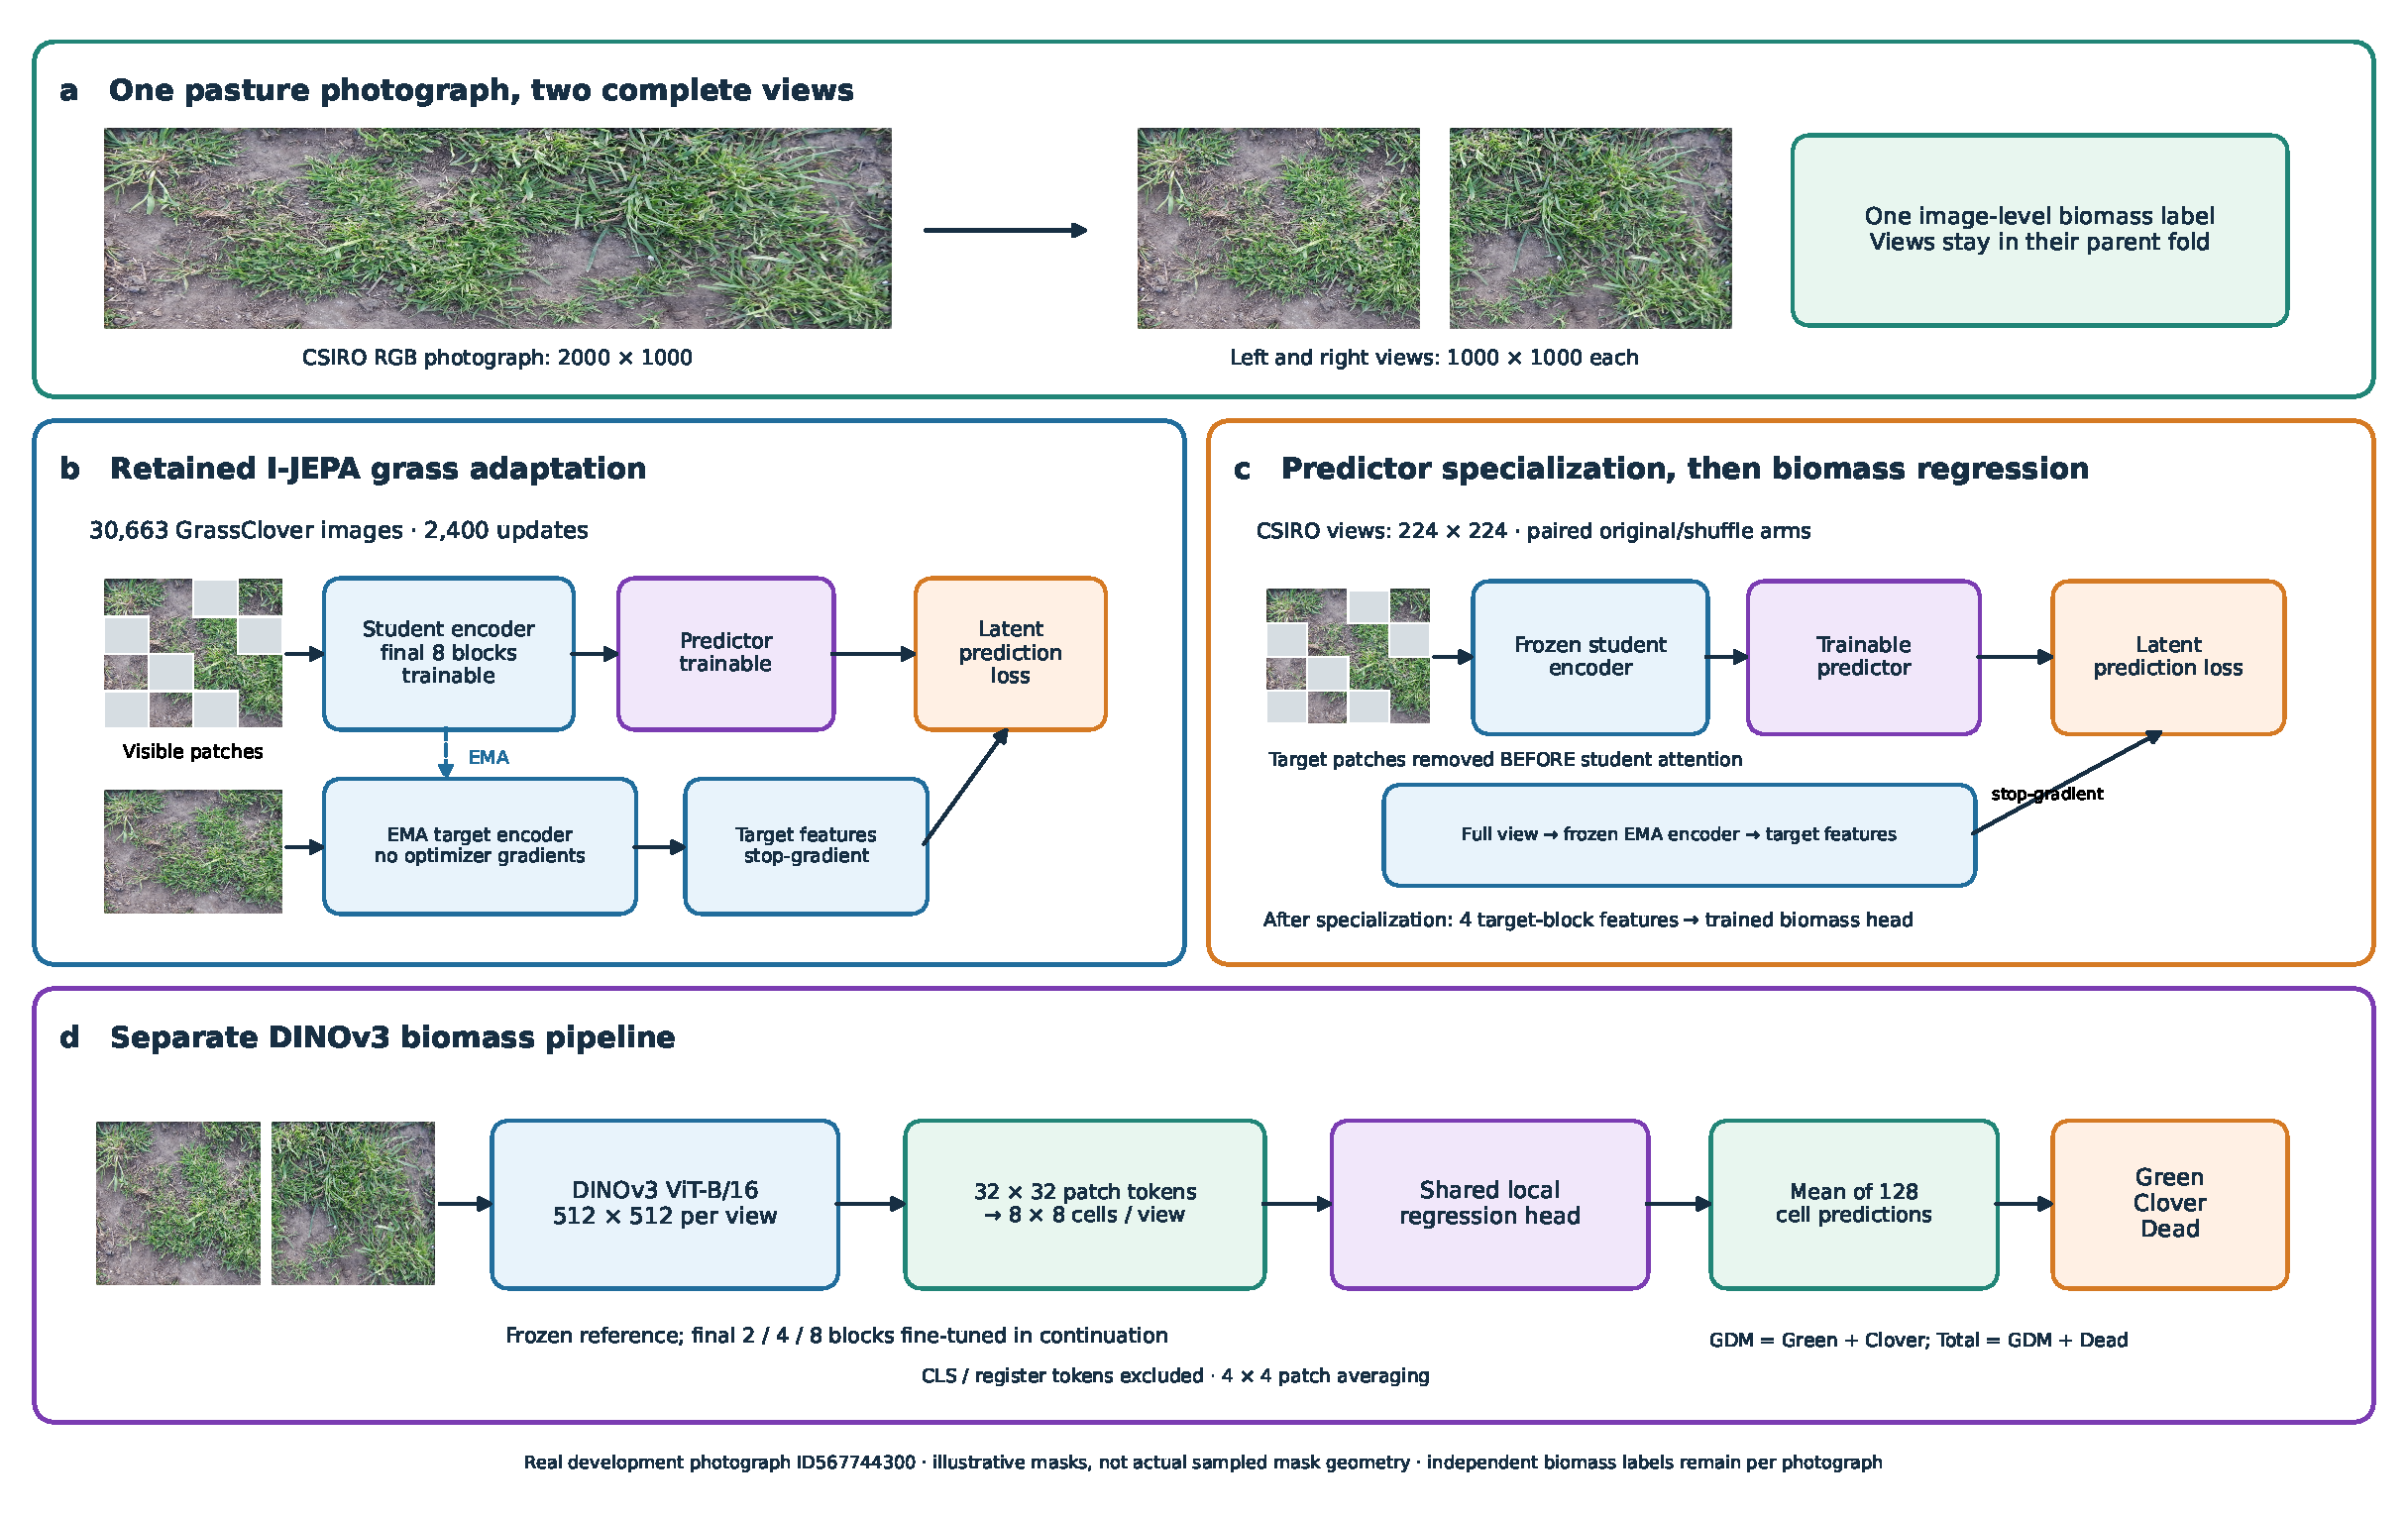
\includegraphics[width=\linewidth]{figures/spatial_pipeline.pdf}
\caption{Image handling and separate transfer stages. (\textbf{a}) A complete CSIRO photograph yields two complete square views; views retain the original fold and image-level labels. (\textbf{b}) Retained grass-domain I-JEPA adaptation updates the final eight student blocks and predictor, with momentum target-encoder updates. (\textbf{c}) Predictor specialization freezes both encoders and compares paired original/shuffled exposures before fitting the biomass head. Hidden target patches are excluded before student attention. (\textbf{d}) DINOv3 aggregates patch embeddings into 128 cells and averages local predictions; continuation unfreezes two, four or eight blocks. Photograph ID567744300 belongs to the reused development evaluation, not an independent test set. It illustrates processing throughout, including panel b; it is not a GrassClover training example. Mask overlays are schematic, not actual sampled masks or semantic target-block geometry.}
\label{fig:overview}
\end{figure}
\begin{figure}[!htbp]
\centering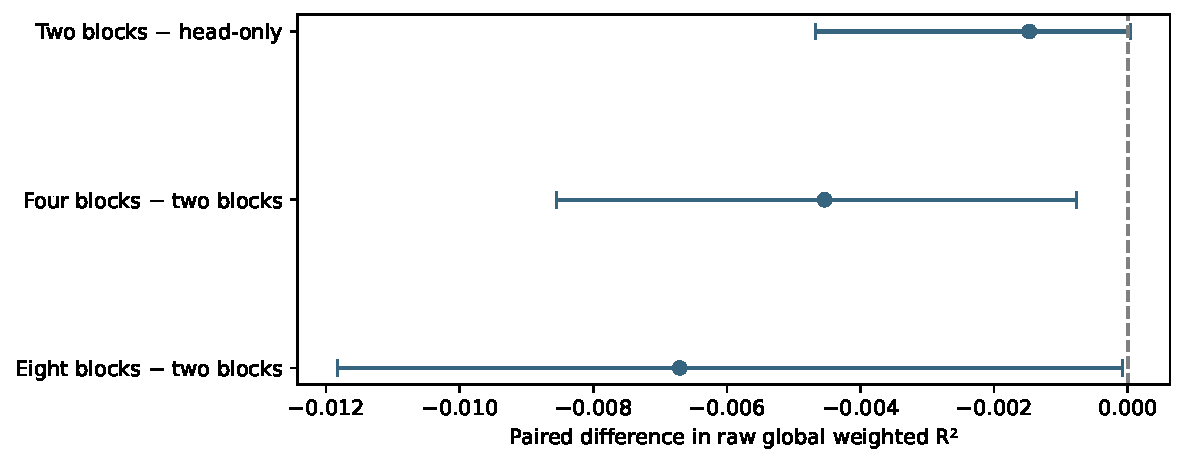
\includegraphics[width=\linewidth]{figures/paired_continuation_effects.pdf}
\caption{Paired DINOv3 continuation differences on 105 photographs from nine acquisition dates. Bars show conditional, unadjusted 95\% intervals from 10,000 paired date-group bootstrap draws; the dashed line indicates zero difference. These intervals exclude seed variability and repeated development selection.}
\label{fig:comparisons}
\end{figure}
\begin{figure}[!htbp]
\centering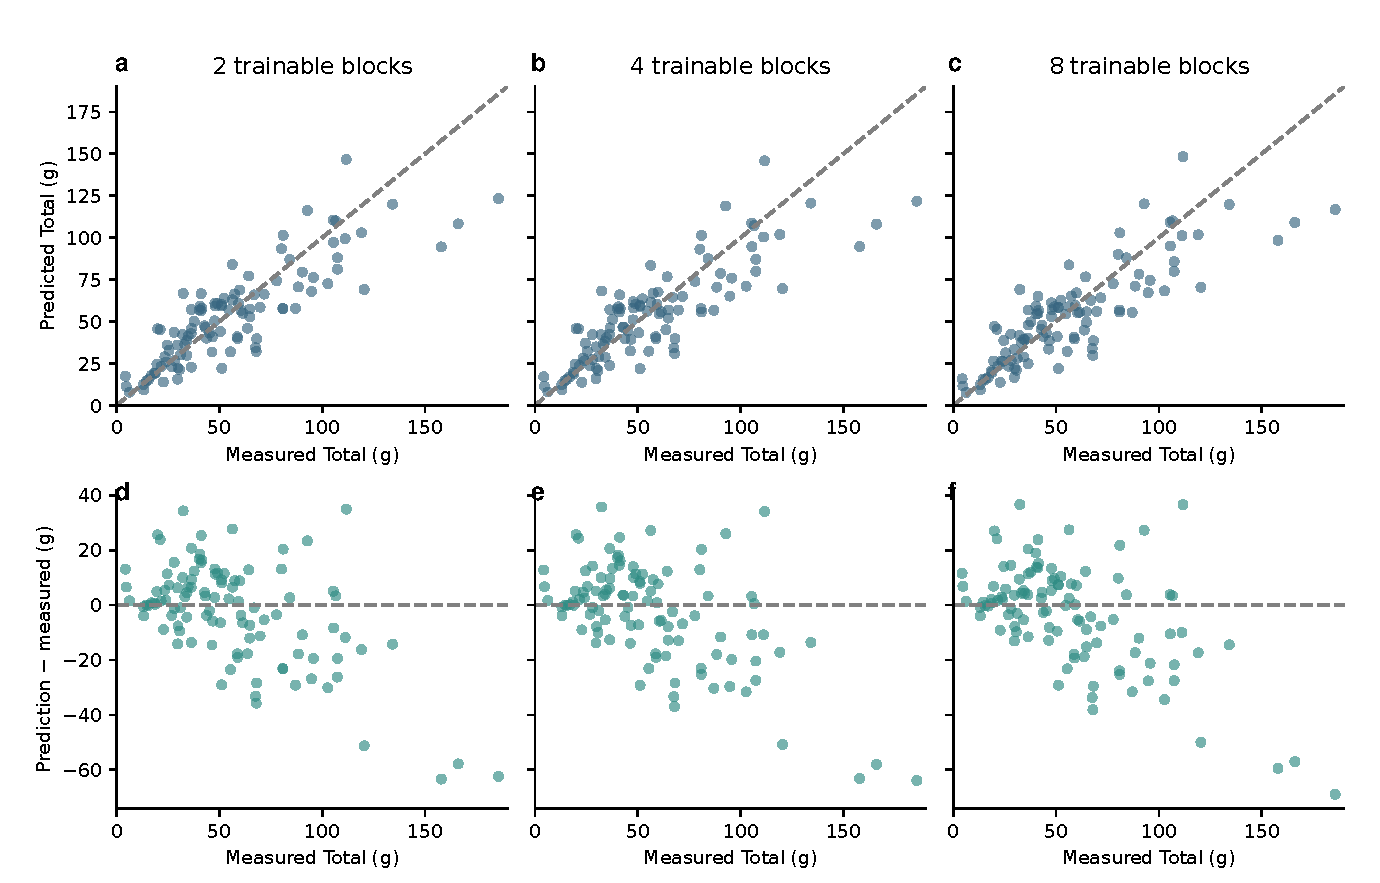
\includegraphics[width=\linewidth]{figures/depth_error_analysis.pdf}
\caption{Measured versus predicted Total biomass and Total residuals for the three DINOv3 adaptation depths. More trainable blocks did not improve the tested recipe; component-specific behavior differs from the global weighted metric.}
\label{fig:depth}
\end{figure}

\subsection{Model sensitivity examples}
Three randomly sampled development photographs were examined with each depth model (nine cases, all fold one). CPU FP32 sensitivity maps and occlusions are retained in Supplementary Figs.~S4--S6 and S10. Four gradient-ranked cells changed Total prediction more than four random cells in six of nine cases, so the ranking was not consistently informative. CPU and saved GPU predictions differed by up to 2.41367~g; GPU attribution stability remains untested. Displayed local contributions are raw head outputs divided by 128 and reconstruct photograph predictions arithmetically, without validating measured local biomass. Historical examples without verified original fold membership are excluded from all main performance comparisons. These diagnostics do not identify a mechanism.

\begin{figure}[!htbp]
\centering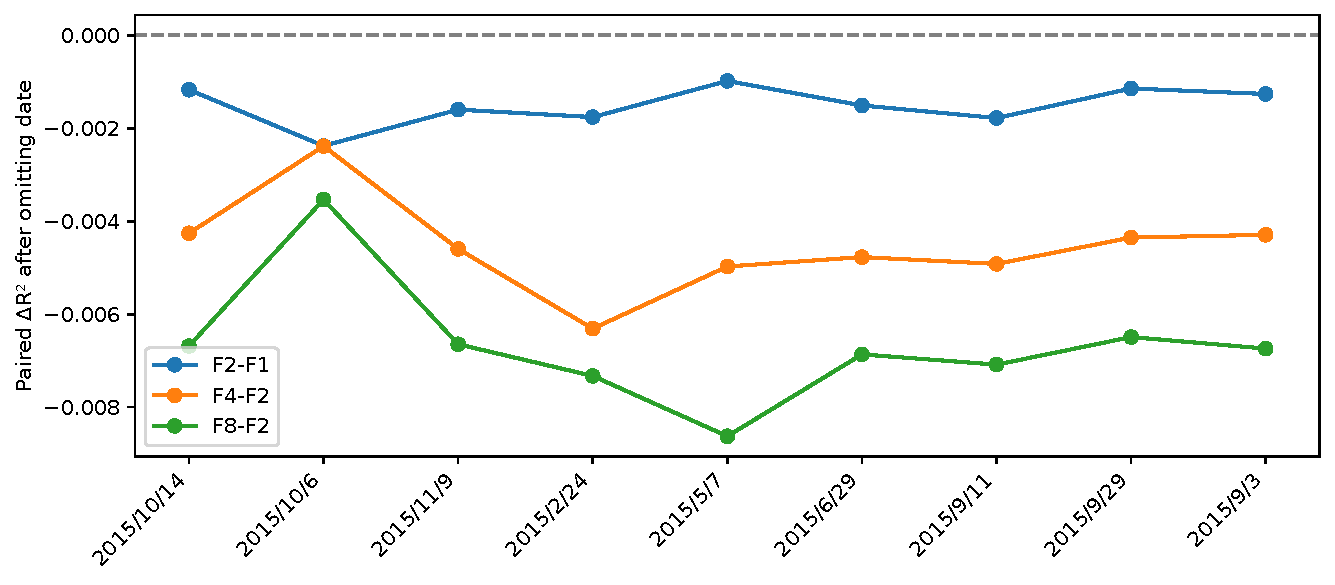
\includegraphics[width=\linewidth]{figures/date_influence.pdf}
\caption{Leave-one-acquisition-date-out sensitivity of the three DINOv3 contrasts. Each point recomputes the pooled score after removing all images from the named date, without retraining. All nine differences retain their original negative signs, but this diagnostic remains conditional on saved models and repeatedly used observations.}
\label{fig:dateinfluence}
\end{figure}

\begin{figure}[!htbp]
\centering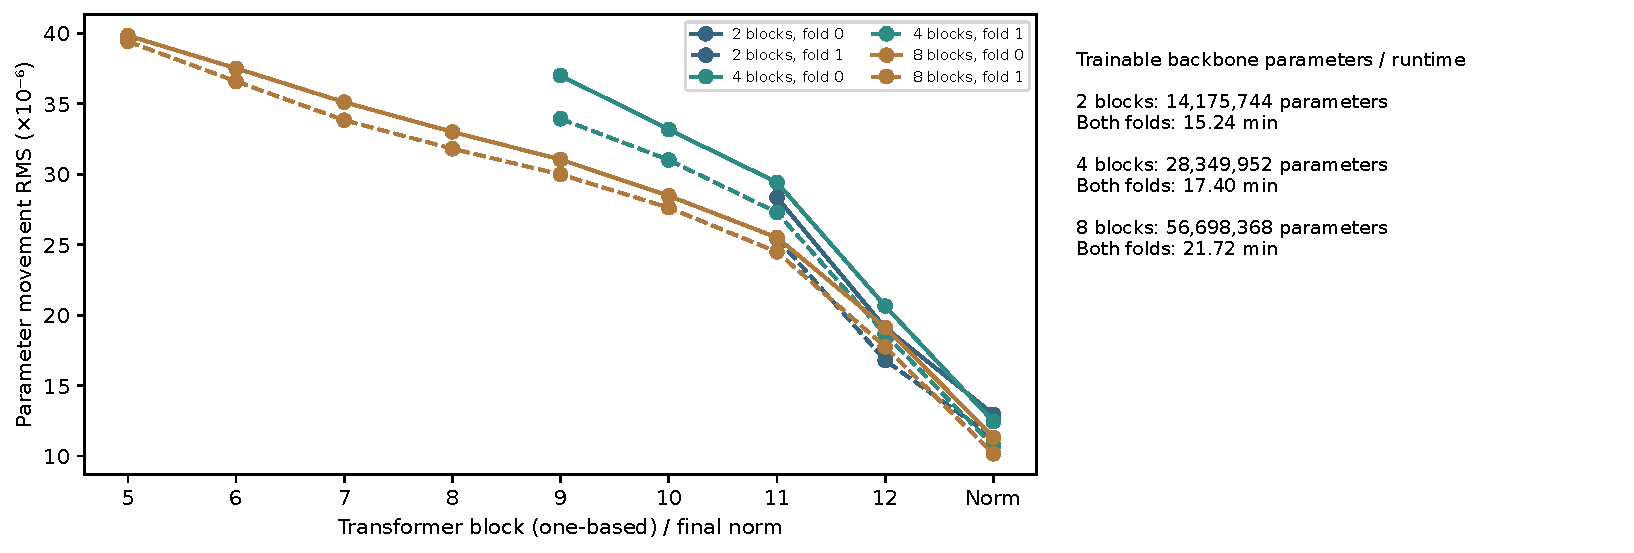
\includegraphics[width=\linewidth]{figures/depth_movement.pdf}
\caption{Measured movement from the pretrained FP32 reference by transformer block and final normalization. Solid and dashed curves distinguish folds. Reported parameter counts and elapsed optimization times are from completed saved runs. Different depths change both trainable capacity and the per-parameter anchoring gradient; these observations do not isolate a causal depth effect.}
\label{fig:movement}
\end{figure}
\begin{figure}[!htbp]
\centering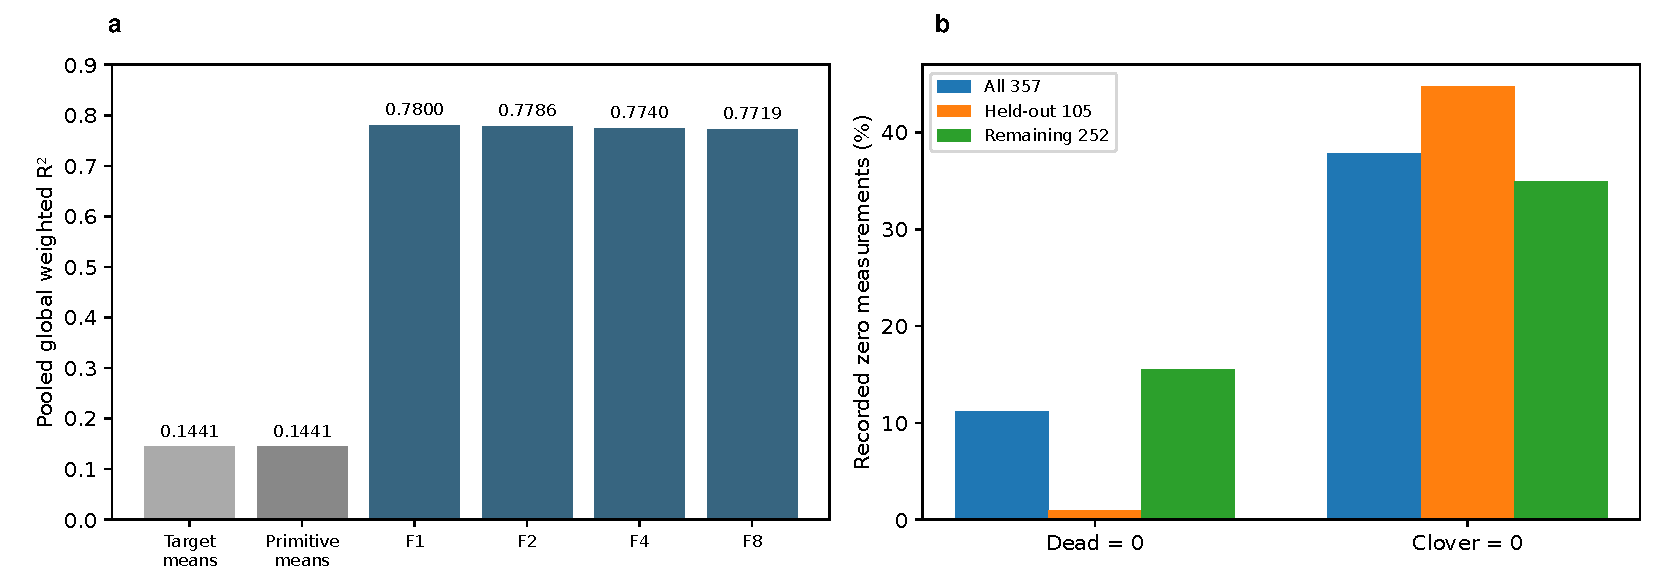
\includegraphics[width=\linewidth]{figures/baseline_and_distribution.pdf}
\caption{Image-free training-only constants versus DINOv3 continuation scores, alongside exact-zero Dead and Clover frequencies. All model scores pool the same 105 development observations. Zero-frequency groups distinguish all 357 photographs, the 105 held-out development photographs, and the remaining 252 photographs; dates were grouped, so no independent-image significance test is implied.}
\label{fig:baselinedistribution}
\end{figure}

\section{Discussion}
For image-based pasture biomass estimation under the evaluated development protocols, frozen DINOv3 dense readouts achieved higher development scores than the examined official I-JEPA readouts, and the tested DINOv3 continuation recipe did not benefit from unfreezing more than two blocks. The evidence supports these narrow observations only. DINOv3 ViT-B/16 and official I-JEPA ViT-H/14 differ substantially in model size, pretraining objective and corpus, patch size, input resolution, and feature readout. In addition, the I-JEPA representations include an adapted model lineage and distinct predictor feature definitions. Thus, the score difference is a comparison of complete transfer pipelines rather than an experiment isolating which pretraining objective is superior.

The I-JEPA results illustrate why a useful adaptation cannot be inferred from its training procedure alone. The grass-adapted encoder outscored the original encoder under the selected frozen-head readout, while a complementary-mask adapted-predictor readout was lower. The more controlled predictor-specialization experiment produced only a small point advantage for the shuffled arm, with an interval spanning negative and positive differences. In another setup, frozen-encoder block permutation had lower point estimates than its no-shuffle control. These outcomes are not contradictory tests of one hypothesis: they use different interventions, folds, readouts, and sample sizes. Collectively they do not justify a general claim that spatial shuffling helps or harms biomass regression.

The JEPA findings concern a bounded transfer protocol, not the capability of the JEPA family in general. The retained adaptation comprised 2,400 updates on 30,663 grass images; subsequent predictor specialization comprised 385 or 377 updates per arm and fold. We did not vary JEPA adaptation duration or biomass-supervised encoder fine-tuning in these comparisons. Large-scale pretraining is a different setting: I-JEPA reports ViT-H/14 training on 16 A100 GPUs in under 72 hours \cite{assran2023ijepa}; VL-JEPA reports four weeks on 192 H200 GPUs, approximately 129,024 aggregate GPU-hours \cite{chen2025vljepa}. VL-JEPA also reports gains with increasing sample exposure in a controlled vision-language experiment. These results establish neither a compute threshold nor an expected biomass gain. GPU-hours across architectures and hardware are not directly comparable. Limited transfer training may be relevant here, but its contribution to the observed score ordering remains untested.

Within the DINOv3 dense-readout study, moving from global pooling to spatial contribution outputs increased the point estimate, but the conditional interval included zero. The feature-aggregation penalty changed the score by less than two ten-thousandths. Its numerical similarity to D1 suggests little measured separation on this development set, not equivalence on unseen data. The local outputs are constrained to aggregate into photograph-level predictions and trained only with photograph-level labels. Without spatially resolved destructive measurements, their values cannot be interpreted as grams of biomass in a cell, nor can they be used to identify species or causal visual evidence.

The depth comparison is similarly specific. It tested a fixed learning rate, fixed 20-epoch schedule, common dense head, and mean-normalized squared-distance penalty to the pretrained weights. The anchoring term was defined as a mean over trainable pretrained parameters, so its aggregate scale changes as the number of trainable blocks changes. Consequently, increasing depth also changes the effective regularization contribution. The observed decline with depth cannot be attributed to the number of blocks alone. Other schedules, unfreezing patterns, anchors, or more target data could produce different outcomes. The result is still useful for the implemented recipe: additional trainable parameters and compute did not improve the prespecified final-epoch global weighted $R^2$ on these reused development folds.

Performance varied by target. Green and total mass were predicted more successfully than Dead mass by per-target $R^2$, while Total residuals in the selected high-mass tail were negative. The weighted aggregate assigns half of the total loss weight to Total, so a favorable aggregate does not imply uniformly accurate component estimates. All component values originate from photograph-level labels; observed accounting identities between Green, Clover, Dead, GDM, and Total are not always exact in source records. We retained recorded labels rather than silently correcting them. The prediction head enforces a compositional relationship among predicted primitives, which can regularize outputs but cannot resolve measurement inconsistency or ecological ambiguity.

The sensitivity analyses provide a limited check on model dependence. Gradient magnitude highlights changes to the model output under infinitesimal input perturbation \cite{simonyan2014saliency}, while occlusion evaluates finite changes under a chosen replacement rule \cite{zeiler2014occlusion}. Neither is a direct measure of causal importance. The disagreements among top-ranked and random occlusions, CPU-versus-training-precision differences, and tiny number of examples make strong interpretive claims inappropriate. The historical DINO-backed JEPA-style lineage has unverified original held-out membership and is documented only in a supplementary provenance note. We include the verified DINOv3 depth-model maps to document what was computed and to motivate cautious reading of visually persuasive explanations, not as biological evidence.

Several design features further limit inference. The 105-image sample is reused and has been consulted repeatedly during model development. Nine acquisition-date groups provide little support for a stable estimate of between-group variability. Dates serve as proxies and are not verified sites; images collected on one date may not capture site, season, management, or instrument diversity. A single training seed leaves optimization variability unmeasured. The bootstrap resamples dates conditional on these saved predictions, and hence does not include retraining, model selection, repeated-fold reuse, or domain shift. The separate 167-image study uses three reused folds and should not be mixed with the 105-image comparisons. None of these scores is a protected independent test result.

Historical competition submissions used different pipelines and do not provide a matched evaluation of these depths. Their score snapshots are recorded separately in the supplementary provenance artifacts.


Further progress should prioritize evaluation design over adding architectural complexity. A locked acquisition-group evaluation, with the split fixed before model selection, would address repeated development reuse. Replication over several seeds would quantify training variability; broader site and season coverage would test domain transfer. If spatial contribution outputs are intended to represent biomass distribution, paired spatially resolved biomass measurements are needed. Code, source versions, licenses, weights, and image-use permissions must also be traceable before independent reproduction or redistribution. These are directions for future work, not completed parts of this study.

The I-JEPA findings are bounded by the available data and tested compute budget. Grass-domain adaptation improved the encoder readout from 0.54649 to 0.58601, whereas predictor reshuffling did not establish a benefit over its matched control. The lower predictor-readout score does not identify its cause or establish general failure of JEPA. Longer adaptation and larger, more diverse datasets remain hypotheses for future controlled evaluation; additional compute alone is not evidence of an expected biomass gain.

\subsection{Conclusion}
For the specific development protocols examined here, frozen DINOv3 dense regression outscored the evaluated official I-JEPA readouts, while the tested increase in DINOv3 unfreezing depth did not improve the two-block reference. Depth also changes the effective per-parameter anchoring strength under the mean-normalized penalty, so this is a result for a fixed recipe rather than a depth-only causal effect. Predictor permutation showed no resolved benefit, and a separate block-shuffle augmentation had lower point estimates than its control. The image-free baselines, markedly different Dead-zero prevalence, shared development data, limited date groups, single seed, and differing model pipelines prevent claims of independent generalization or objective-level superiority. These results support careful, matched evaluation of pretrained representations for biomass estimation and further data collection before stronger biological or deployment conclusions.

\section{Methods}
\subsection{Data and target definitions}
We used the competition-provided 357 publicly labeled CSIRO training photographs with nominal dimensions of $2000\times1000$ pixels. These form a subset of the larger 1,162-image source dataset described by Liao et al. \cite{Liao2025PastureDataset}; hidden competition images were not used for supervised training. Five image-level target values are reported in grams: Green dry mass (\texttt{Dry\_Green\_g}), dead dry mass (\texttt{Dry\_Dead\_g}), clover dry mass (\texttt{Dry\_Clover\_g}), green dry matter (\texttt{GDM\_g}), and total dry mass (\texttt{Dry\_Total\_g}). For training, the models predict three nonnegative primitive quantities, Green ($G$), Clover ($C$), and Dead ($D$), and derive $\widehat{\mathrm{GDM}}=\hat G+\hat C$ and $\widehat{\mathrm{Total}}=\hat G+\hat C+\hat D$. This parameterization makes predicted totals internally consistent. Source records were preserved without correction. In all 357 labeled photographs, 135 Clover and 40 Dead measurements were exactly zero; the 105-image evaluation subset contained 47 and one, respectively. One full-dataset Total accounting residual exceeded 0.01~g (maximum 0.3088~g), while none did in the 105-image subset. GDM identity residuals were at most 0.0001~g. Exact zeros are recorded measurements, not independently verified biological absence.

The primary I-JEPA and DINOv3 comparisons used existing folds 0 and 1, grouped by acquisition date. Their training/validation counts were 308/49 and 301/56. The pooled validation predictions cover 105 distinct photographs across nine date groups. A separate frozen I-JEPA augmentation experiment used folds 0, 1, and 2, comprising 167 photographs and 14 acquisition dates. All folds were reused during development; there was no protected test set for these analyses. Grouping is appropriate when observations share temporal or spatial structure \cite{roberts2017crossvalidation}. Date grouping separates photographs from the same recorded date but does not establish independence by site, season, or management. No image crop or transformed copy is treated as an independent biological sample.

GrassClover supplied 30,663 unlabeled images for the retained I-JEPA adaptation. Its image-level composition annotations were not used to create additional CSIRO biomass labels. Only the five CSIRO targets enter the reported biomass regression metrics. The images and labels retain their source-specific provenance and redistribution conditions.

\subsection{Primary metric and uncertainty}
The primary endpoint pools all held-out predictions and labels and computes one raw global weighted coefficient of determination:
\begin{equation}
R_w^2=1-\frac{\sum_{i=1}^{N}\sum_{t=1}^{5}w_t(y_{it}-\hat y_{it})^2}{\sum_{i=1}^{N}\sum_{t=1}^{5}w_t(y_{it}-\bar y_w)^2},\qquad
\bar y_w=\frac{\sum_{i,t}w_ty_{it}}{\sum_{i,t}w_t}.
\end{equation}
Target weights in Green, Dead, Clover, GDM, Total order are $(0.1,0.1,0.1,0.2,0.5)$. This is not the mean of fold-specific $R^2$, mean target $R^2$, or an $R^2$ computed after logarithmic transformation. For the image-free baselines, each validation fold receives constants estimated solely from the corresponding fold-specific training partition. The five-target baseline averages each recorded target separately. The consistent baseline averages the three primitives and derives the other two constants by summation. Training and held-out image IDs and acquisition dates are disjoint in each fold; pooled scoring uses the same 105 observations as the image models. Secondary metrics are MAE and RMSE, reported in grams, and target-specific $R^2$, which is dimensionless. Exploratory intervals are unadjusted for multiple comparisons. Bootstrap resampling provides a general empirical uncertainty procedure \cite{efron1979bootstrap}. Here, intervals use 10,000 paired resamples of acquisition-date groups, carrying all images within a sampled group. They describe conditional variation among the nine or fourteen observed groups for the saved predictions; they do not quantify seed uncertainty or correct repeated development use.

\subsection{Official I-JEPA representations and frozen-backbone regression protocol}
The official I-JEPA source is ViT-H/14 with a 32-block encoder with 1,280-dimensional embeddings and a paired 12-block predictor with internal width 384. The source code was pinned to the official repository revision recorded in the project provenance. The retained grass-domain adaptation used 2,400 optimizer steps on the 30,663-image unlabeled corpus, updated the final eight student encoder blocks and the predictor, and maintained a momentum target encoder. The adapted encoder and predictor weights were retained for downstream readout. The adaptation experiment is not the same as supervised biomass fine-tuning.

Each original $2000\times1000$ photograph was represented by two complete, non-overlapping square halves of $1000\times1000$ pixels, resized to $224\times224$. The official encoder has no CLS token, so patch features were mean-pooled per view. The frozen encoder regression head maps each view through layer normalization and a 512-unit linear/GELU projection, then gated attention combines the two views. A 512-to-256 layer with GELU and dropout feeds three positive primitive outputs. The complementary-mask predictor reference uses its saved predicted-latent representation and is reported as its own readout; it is not treated as interchangeable with the later semantic target-block specialization.

For the frozen-backbone regression study, the global loss is raw weighted mean squared error divided by the square of a single training-fold scale. The scale and output medians are computed from training labels only. Heads use AdamW \cite{loshchilov2019adamw} with learning rate $3\times10^{-4}$ and weight decay 0.01 for 200 epochs. The selected checkpoint is the average of the final 40 epoch weights, not the epoch with the highest validation score. Training uses only the four right-angle rotations of the preprocessed square views; validation uses identity orientation. Rotations are pixel permutations and remain attached to their parent image and fold. No reflection, arbitrary-angle rotation, crop, or photometric augmentation is used in this protocol.

\subsection{Predictor specialization and block permutation}
For the predictor-specialization experiment, the student and EMA encoders were frozen, and target patches were removed before student attention. The unshuffled and shuffled arms shared the initial adapted predictor, actual materialized context/target masks, image exposure schedule, optimizer recipe, and downstream head. The shuffled arm used ten within-image $10\times10$ block permutations. Each block permutation remained within its source photograph. The two arms completed 385 and 377 predictor updates in folds 0 and 1, respectively. The semantic readout exposes 88 of 256 patches per view (34.375\%); four target regions contain the remaining 168 patches (65.625\%). Downstream regression used four fixed 42-token semantic target-block readouts from the specialized predictor and the common frozen-backbone regression training protocol. The complementary-mask predictor reference described above has a different readout construction and is therefore not this experiment's unshuffled comparator.

The separate frozen-encoder augmentation experiment compared no block permutation with $4\times4$ and $10\times10$ permutations. On each full view, a permutation was applied before resizing with training probability 0.35; validation data remained unchanged. All arms used the same frozen grass-adapted encoder, a shared gated regression head, raw weighted MSE, and the three-fold 167-image development split. Permutations alter training exposures but do not increase the number of independent photographs.

\subsection{DINOv3 dense feature regression}
The DINOv3 backbone is the official ViT-B/16 model with 12 transformer blocks and 768-dimensional patch features. Each complete square view was resized by bicubic interpolation to $512\times512$ and normalized using ImageNet channel statistics. The $32\times32$ patch grid excluded CLS and register tokens. Averaging disjoint $4\times4$ patch groups produced an $8\times8$ spatial feature map for each view. Equal-area averaging of cell predictions over both views produced photograph-level outputs.

D0 uses globally pooled features and a global regression head. D1 and D2 use a shared linear--GELU--linear local head with dimensions $768\to256\to3$ and softplus primitive outputs scaled by a training-fold scalar. For target $t$, let $a_{v,r,c,t}$ denote the raw local-head prediction for target $t$ at row $r$, column $c$, in view $v$ (with derived targets formed by the same primitive sums). With two views and $8\times8$ cells per view,
\begin{equation}
\hat y_t=\frac{1}{128}\sum_{v=1}^{2}\sum_{r,c=1}^{8}a_{v,r,c,t},\qquad q_{v,r,c,t}=\frac{a_{v,r,c,t}}{128}.
\end{equation}
The displayed $q$ values sum to $\hat y_t$; raw $a$ values do not. The plotted $q$ values are model-derived, normalized contributions whose sum equals the image-level prediction in grams. These are contribution proxies rather than externally measured grams per cell. D0, D1, and D2 are trained on the same two-fold development sample. D1 optimizes the biomass objective alone, whereas D2 also matches fine-grid predictions to predictions from features coarsened to a $4\times4$ grid. Both grids derive from a single 512-pixel encoder stream; no second image resolution is encoded:
\begin{align}
L_{\mathrm{bio}}&=\frac{1}{Ns^2}\sum_{i=1}^{N}\sum_{t=1}^{5}w_t(y_{it}-\hat y_{it})^2,\\
L_{\mathrm{D2}}&=L_{\mathrm{bio}}+0.10\frac{1}{3Ns^2}\sum_{i=1}^{N}\sum_{t=1}^{3}(\hat y^{\mathrm{fine}}_{it}-\hat y^{\mathrm{coarse}}_{it})^2.
\end{align}
The executed feature cache used identity orientation only. D1 and D2 have identical inference architecture; their distinction is the training loss.

\subsection{DINOv3 continuation and anchoring}
Depth arms start from the same official pretrained backbone and the fold-specific saved D2 head and scale. In the depth comparison, the final two, four, or eight transformer blocks and output normalization are trainable; earlier blocks remain frozen. The two-block reference is independently trained as part of this study. Each arm uses 20 epochs, a batch size of two photographs and gradient accumulation across eight batches, AdamW with $\beta_1=0.9$, $\beta_2=0.999$, and $\epsilon=10^{-8}$, cosine epoch-wise learning-rate decay, and gradient clipping at norm one. The head learning rate is $3\times10^{-5}$ and backbone learning rate $2\times10^{-6}$. Head weight decay is 0.01 and backbone weight decay is zero. Each training photograph is used once each epoch, including the final partial accumulation window. The selected model is the fixed final-epoch checkpoint rather than a validation-selected checkpoint.

Pretrained anchoring is the mean squared distance over trainable pretrained parameters, $L_{\mathrm{SP}}=P^{-1}\sum_p(\theta_p-\theta_p^{(0)})^2$, with total loss $L=L_{\mathrm{D2}}+10^6L_{\mathrm{SP}}$. The anchor values are immutable official pretrained weights. The direct anchoring gradient for parameter $p$ is $2\lambda(\theta_p-\theta_p^{(0)})/P$. Backbone parameter counts for depths two, four and eight are 14,175,744, 28,349,952 and 56,698,368, respectively. Layer-wise pretrained movement is measured from the retained FP32 tensors (Fig.~\ref{fig:movement}). The coefficient and recipe were fixed before the completed run. Because $L_{\mathrm{SP}}$ is normalized by the number of trainable parameters, its aggregate regularization effect changes with unfreezing depth; the depth comparison is not independent of this feature of the penalty.

\subsection{Execution and artifact verification}
The completed depth study ran on NVIDIA RTX PRO6000 Blackwell hardware with eligible FP8 linear operations, higher-precision remaining operations and FP32 master weights. Saved checks verified intended updates, frozen prefixes, initialization parity, checkpoint reconstruction and metric arithmetic. Source hashes, environment records, resume checks and prediction manifests are retained in the review artifacts. These engineering checks do not provide independent validation.

\subsection{Sensitivity analysis}
For DINOv3 depth examples, three original photographs were sampled uniformly without replacement from the 105 validation photographs using seed 42. All belonged to fold one. The fold-one checkpoints for depths two, four, and eight were reconstructed and evaluated in CPU FP32. Input gradients of the Total output were aggregated as $|x\nabla_x|$ over an $8\times8$ grid in each view. Four highest-ranked cells were occluded and compared with four cells selected at random using a fixed seed. Occlusion replaced normalized inputs with zero, equivalent to channel-mean RGB fill. The same image cases were evaluated at each depth. All 45 target predictions differed between CPU and saved training precision; Total discrepancies ranged from 0.0812 to 2.4137~g (0.253--7.107\% of the saved Total prediction). Relative-error denominators are saved predictions, not measured labels. GPU/CPU attribution agreement was not measured. Saved training-precision predictions are retained alongside CPU values because numerical differences were observed.

The sensitivity analyses are descriptive perturbation tests. They do not establish causal attribution, local biomass, or model faithfulness on a population of images.

\subsection{AI-assisted preparation}
OpenAI Codex was used to assist code implementation, analysis scripting, manuscript drafting and editing. Reported continuation metrics were independently recomputed from preserved prediction arrays, and generated figures were checked against their source data. An image-generation tool assisted conceptual layout exploration for Fig.~\ref{fig:overview}; the final diagram was rendered programmatically from verified protocol labels and an original dataset photograph. Generative image outputs were not used as photographs, measurements or model outputs.

\subsection*{Code availability}
A versioned local reviewer archive (SR-release-r7-authors-2026-10-11) accompanies this draft with source code, configurations, saved prediction tables, fold assignments, verification scripts and SHA-256 manifests. It is not a public release; pretrained and trained weight redistribution remains subject to source terms. The illustrative repository address \url{https://github.com/anonymous-research/pasture-biomass-transfer} is a placeholder and is not a released repository.

\section*{Data Availability}
The labeled photographs are provided through the CSIRO Image2Biomass dataset \cite{csiro2025image2biomass}; GrassClover is described in its dataset publication \cite{skovsen2019grassclover} and is accessible through \url{https://vision.eng.au.dk/grass-clover-dataset/}. CSIRO competition data are accessible through \url{https://www.kaggle.com/competitions/csiro-biomass/data}. Reuse and redistribution are subject to the respective source terms. No new image dataset is released with this study. Publication-use permissions for reproduced photographs require author confirmation before submission.
\bibliography{references}
\section*{Author contributions}
Chandrakala G Raju, Megh Mayur M R, Mohd. Viquaruddin Anas and Karthik N H contributed equally to this work.
\section*{Additional Information}
\subsection*{Competing interests}
The authors declare no competing interests.
\section*{Funding and acknowledgements}
This work was supported by B.M.S. College of Engineering.
\end{document}
